\chapter{Pairing in Nuclear Theory}

\maketitle
There are several different ways to include pairing correlations in nuclear structure calculations, many of which are based on the BCS theory of superconductors. In it, nucleon pairs can be described as quasiparticles in a nuclear superfluid. Here I will describe three different approaches for describing nuclear structure which account for pairing, each with varying degrees of generality.

First I might ask you, though: why should we even do any specific considerations for pairing at all? Shouldn't the nuclear force contain the entire interaction? So then why do we invent things like HF-BCS or HFB where pairing is \textit{separate} from the mean field interaction? Is pairing just an artificial construct? And my answer is that the question is somewhat misleading. Pairing isn't really related to the mean field, or even the nucleon-nucleon interaction. It's actually more a result of the Pauli exclusion principle and quantum orbitals and such. Pairs form when you have two nucleons in the same quantum state, except with opposite spin or isospin. Then they kind of just hang out with each other in the same places and do everything together because that's what pairs in the same quantum state do. So it kind of maybe amplifies the effect of the nucleon-nucleon interaction (or rather, the fact that other nucleons are found in separate orbitals might tend to damp it). This is true for mean field/DFT models; in shell model theories, there's no real need for this distinction (see \cite{???? https://arxiv.org/pdf/1205.2134.pdf}; is pairing even a meaningful concept in shell models?).

Just some terminology: \textbf{Pairing strength} refers to the coefficient of the \textit{effective} pairing interaction. A large pairing strength means pairs are more likely to form. \textbf{Pairing gap} refers to the energy it takes to break a pair and promote one particle to the next energy level. A large pairing gap keeps pairs together. Pairing strength and pairing gap are similar concepts and may be related in some cases; the difference is that one is a phenomenological construct used in effective theoretical descriptions whereas the other is a physically ``measurable'' quantity. \textbf{Pairing energy} refers to the extra binding energy associated with nucleonic pairs. It is (I believe) the energy contribution coming from the effective pairing interaction.

I should also mention that in the literature, there are two types of pairing that get mentioned: static and dynamic pairing correlations. So far as I can tell, \textbf{static pairing} refers to pairing at the level of HF+BCS or HFB. It might, for example, take the form of a density-dependent zero-range interaction such as this:

\begin{equation*}
V(r) = V_0\left(1-\left(\frac{\rho(r)}{\rho_0}\right)^\alpha\right)
\end{equation*}

\noindent I believe this is what you would use to create the $\Delta$ in your HFB matrix, for instance. \textbf{Dynamic pairing} refers to correlations that go beyond this approximation, and they are what cause so-called pairing fluctuations or pairing vibrations (if pairing correlations are strong enough and you start moving away from magic nuclei, the parameters defining the pairing gap will fluctuate or vibrate around their ground state value in the same way the surface shape might vibrate around its ground state shape). Essentially you can break down the energy like this:

\begin{equation*}
E \rightarrow E_{HF} + E^{pair}_{static} + E^{pair}_{dyn} \equiv E_{HFB} + E^{pair}_{dyn}
\end{equation*}

I believe Lipkin Nogami is an example dynamic pairing recipe. In essence, you see pairs becoming more or less attached to their parent nucleus, and that in turn affects the dynamics. This is why Lipkin-Nogami keeps track of particle number: because the particle number of the nucleus is actually somewhat changing, as those pairs decide whether or not to stay attached (and I'm not sure whether I mean the pair would separate or if they would just be excited as a boson-like pair). By fixing the particle number as you do with Lipkin-Nogami, you essentially fix the gap strength, which determines how hard the nucleus has to work to keep that pair attached. Sometimes it'll be worth it, and sometimes it won't.

For more information on static vs dynamic pairing correlations, some possible starting points are this passage from 50 Years of Nuclear Pairing (figures \ref{fig:static_dynamic_pairing1} and \ref{fig:static_dynamic_pairing2}), along with this paper: \cite{SHIMIZU1990c477}. To see how they play a role physically, see \cite{SHIMIZU198733} and \cite{MORETTO19721}.

\begin{figure}
\centering
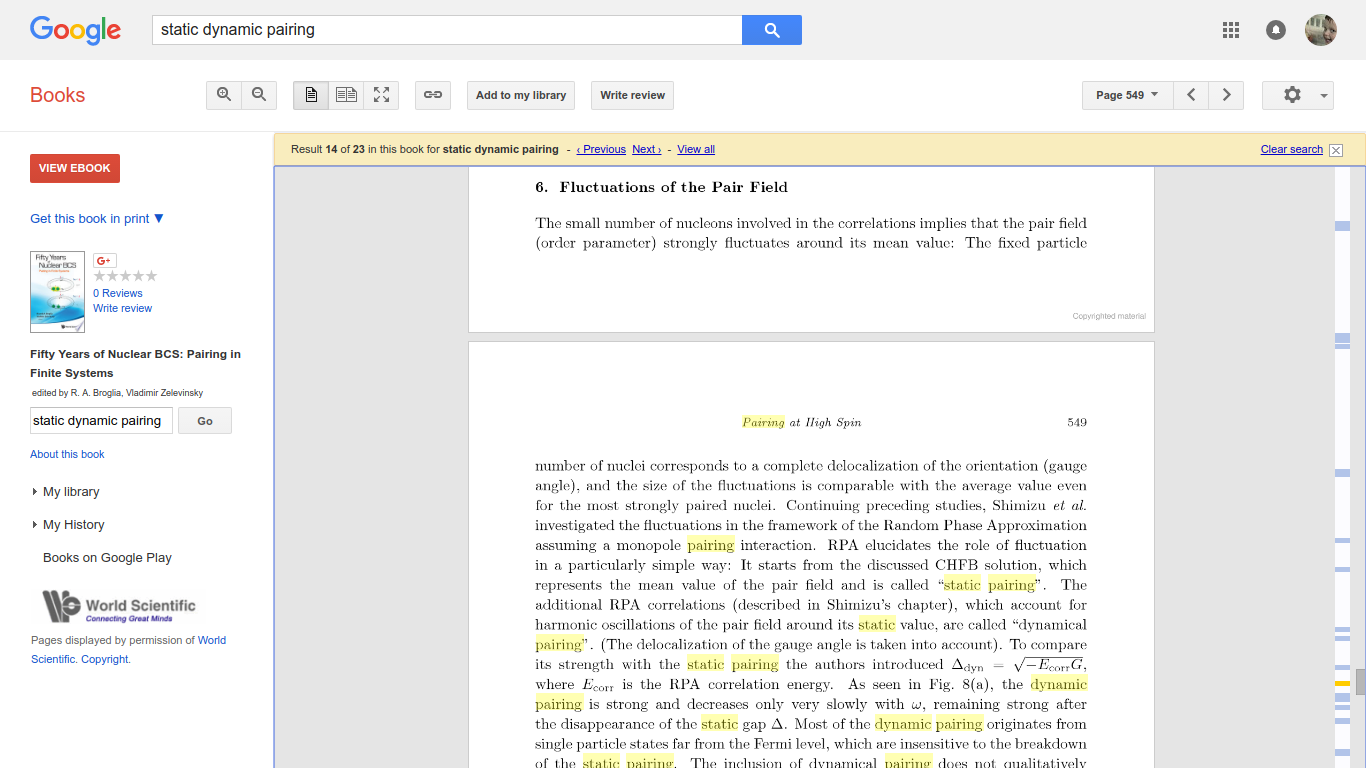
\includegraphics[width=0.7\linewidth]{TeX_files/static_dynamic_pairing1}
\caption{Part 1 of a helpful description of the difference between static and dynamic pairing.}
\label{fig:static_dynamic_pairing1}
\end{figure}

\begin{figure}
\centering
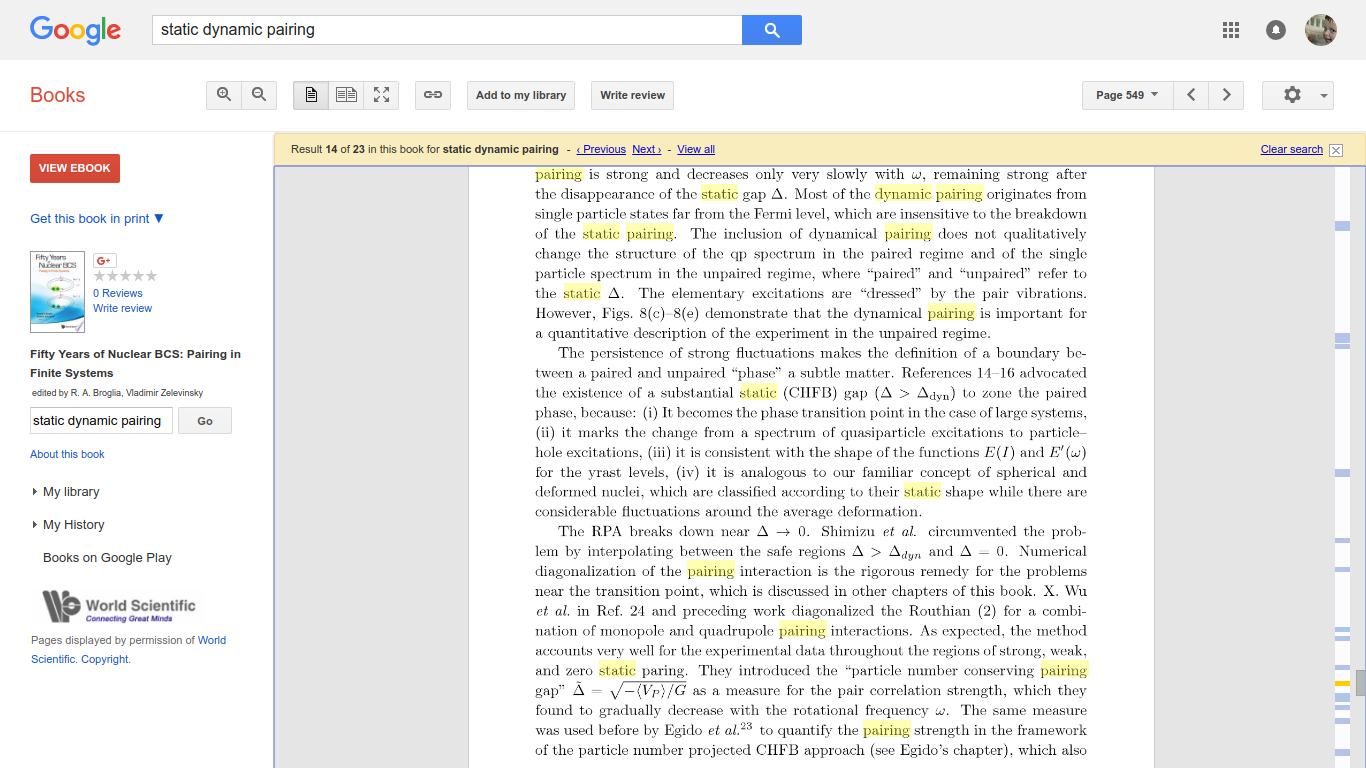
\includegraphics[width=0.7\linewidth]{TeX_files/static_dynamic_pairing2}
\caption{Part 2 of a helpful description of the difference between static and dynamic pairing.}
\label{fig:static_dynamic_pairing2}
\end{figure}


\section*{BCS Theory and HF+BCS (\cite{suhonen2007nucleons,Anguiano2013})}
One way to include pairing correlations is to solve the Hartree-Fock equations and add BCS on top. This method is called HF+BCS and it does a fair job of describing nuclei near the valley of stability, but gets progressively worse the further from stability you get (see \cite{Anguiano2013}).

Basically the idea is that you use HF to take you from a system with a whole bunch of interdependent particles, which each obey a one-body Hamiltonian piece AND a two-body Hamiltonian piece, to an alternate basis in which you basically only have a one-body Hamiltonian. Then, in that basis, you solve the BCS equations on top, so you're doing BCS on a basis that doesn't exactly describe the real interaction Hamiltonian but is close enough to the real thing.

Another way of saying it is that the HF equations give you single-particle wavefunctions, in the basis which most closely approximates/diagonalizes the [two-body] Hamiltonian. So it's sort of a fictitious basis, in that your Hamiltonian is not \textit{really} diagonal, but it's as good as you're gonna get. That's what the variation does - you're varying the ground state energy according to the coefficients which give you the most ideal linear combination of starting basis functions (harmonic oscillator or whatever). But the main idea is this: that you pretend your two-body Hamiltonian is actually a one-body Hamiltonian, diagonalize it, and make the error in your approximation as small as possible.

For the next step, when you add in the BCS, you typically make (at least for even-even nuclei) the ground state ansatz $|BCS\rangle = \prod_{k>0}(u_k+v_k a_k^\dagger a_{\bar{k}}^\dagger)|0\rangle$, which doesn't conserve particle number (in fact, it's a linear superposition of pairs starting from zero pairs all the way up to $\frac{A}{2}$ pairs), but I guess it's close enough. Then you typically enforce particle number conservation some other way, perhaps by adding a Lagrange multiplier.

Next you take your pairing Hamiltonian, which I suppose would include your mean-field, now one-body Hamiltonian (which stands in for the two-body Hamiltonian you had before you performed Hartree-Fock), and you add in a new two-body potential, which this time represents the effect of pairing. Then you perform a Hartree-Fock-style calculation all over again, essentially just doing another Hartree-Fock calculation on top of your original one, except that this time you might probably have an extra Lagrange multiplier constraint in your Hamiltonian. It doesn't change anything substantial but it's good to keep in mind. There are probably other ways of constraining particle number, too, like Lipkin-Nogami, but I'm not too sure how those work.

Some other things to keep in mind:
\begin{itemize}
\item You can still think of your system in terms of the HF-basis real particle wavefunctions $a_k^\dagger |0\rangle$, with $|BCS\rangle = \prod_{k>0}(u_k+v_k a_k^\dagger a_{\bar{k}}^\dagger)|0\rangle$. Or, to simplify the math, you can invent a new "quasiparticle" such that $|BCS\rangle = \prod_{k}\alpha_k^\dagger|0\rangle$. This trick is called the Bogoliubov transformation and it looks like this:

\begin{eqnarray}
\alpha_k^\dagger = u_ka_k^\dagger-v_ka_{\bar{k}} \label{quasiparticle1}\\
\alpha_{\bar{k}}^\dagger = u_ka_{\bar{k}}^\dagger+v_ka_k \label{quasiparticle2}
\end{eqnarray}
\item A pairing gap $\Delta = 0$ seems to mean there is no energy associated with pairing. All pairs are formed below the Fermi surface, because why on Earth wouldn't they? It's free! Whereas a nonzero pairing gap means there is some energy associated with forming a pair. So the probability of forming pairs is less than one below the Fermi surface, but there's also a possibility that pairs might form outside the Fermi surface. The pairing gap basically defines how far outside the Fermi surface you can go (see p 233 of \cite{ring1980nuclear}, for ex., or p 13 of \cite{Balbuena2003}).
\item You could also do the BCS calculation using single-particle states derived from a phenomenological potential. You'd sacrifice some accuracy but gain some speed \cite{Anguiano2013}.
\end{itemize}

\section*{Hartree-Fock-Bogoliubov (HFB)  (\cite{ring1980nuclear,Balbuena2003})}
In HF theory, you find the eigenfunctions of the one-body Hamiltonian which most closely resembles the actual two-body Hamiltonian. The basic idea to HFB is that in HFB you do basically the same thing, except you can't ignore two-body interactions because of pairing. So I guess in a way you sort of find the eigenfunctions of the two-body Hamiltonian which most closely resembles the actual four-body Hamiltonian. There's a little bit more subtlety than that, because the pairing correlations mean the particles are related somehow, but that's not a bad way to envision it, because one quasiparticle has a $U$ term, which corresponds to adding a particle, and a $V$ term, which does the opposite - so it's like creating a pair all at once (see equation \ref{HFBqp})! In reality, each HFB quasiparticle is a sum of such terms, but you get the idea. In some sense, one quasiparticle $\sim$ two real particles.

By way of comparison to HF+BCS, which is a two-step process, HFB just does both steps at once to give you a single set of quasiparticle wavefunctions, instead of one set of single-particle wavefunctions based on another set of wavefunctions. The approximation in the end is better, but it is more computationally intensive than HF+BCS.

Let's see how this calculation is to be done. Suppose our Hamiltonian is:

\begin{equation}
\hat{H}=\sum\limits_{i,j} t_{ij} \hat{c}_i^\dagger \hat{c}_j + \frac{1}{4}\sum\limits_{i,j,m,n} \bar{v}_{ijmn} \hat{c}_i^\dagger \hat{c}_j^\dagger \hat{c}_n \hat{c}_m
\end{equation}

As mentioned before, let us make the following Bogoliubov transformation to make the math simpler:

\begin{equation}
\left(\begin{array}{c}
\hat{\beta} \\
\hat{\beta^\dagger}
\end{array}\right)
= \left(\begin{array}{cc}
U^\dagger & V^\dagger \\
V^\dagger & U^\dagger
\end{array}\right) \left(\begin{array}{c}
\hat{c} \\
\hat{c^\dagger}
\end{array}\right) \label{HFBqp}
\end{equation}

\noindent Now the Hamiltonian looks like this:

\begin{eqnarray}
\hat{H} = \hat{H}_0 + \sum\limits_{i,j}\hat{H}_i,j\beta_i^\dagger\beta_j + \sum\limits_{i<j}(\hat{H}_{i,j}\beta_i^\dagger\beta_j^\dagger + h.c.) + \hat{H}_{int} \nonumber\\
= \hat{H}_0 + \hat{H}_{11} + \hat{H}_{20} + \hat{H}_{40} + \hat{H}_{31} + \hat{H}_{22}
\end{eqnarray}

\noindent where $h.c.$ is the hermitian conjugate of the previous term and the term $\hat{H}_{nm}$ contains all terms with $n$ quasiparticle creation operators and $m$ annihilation operators. We'll lump the terms with 4 creation/annhilation operators into a single term $\hat{H}_{int}$, which we'll assume is small and thus ignore (sort of like the term $V(r)-\sum_{i,j}V(r_i,r_j)$ from regular Hartree-Fock theory). Let us constrain the average particle number by adding in a Lagrange multiplier term $\lambda N$. Then we vary the total energy with respect to $U$ and $V$ (which are matrices):

\begin{equation}
\delta E' = \langle\Phi_0|\hat{H}-\lambda\hat{N}|\Phi_0\rangle
\end{equation}

After that, it's really just algebra. The variation leaves some ambiguity still in the choice of $U$ and $V$, so we will choose them to make $\hat{H}_{20}=0$ and $\hat{H}_{11}$ diagonal. Additionally, the solution will look nicer if we introduce the following two densities, the traditional single-particle density from Hartree-Fock $\rho$ and a pairing tensor called $\kappa$:

\begin{eqnarray}
\rho_{ij} = \langle\Phi_0|\hat{c}_j^\dagger\hat{c}_i|\Phi_0\rangle = (VV^T)_{ij} \\
\kappa_{ij} = \langle\Phi_0|\hat{c}_j\hat{c}_i|\Phi_0\rangle = (VU^T)_{ij}
\end{eqnarray}

\noindent I'd just like to mention something here that Nicolas also mentions in his notes: that you can think of the single-particle density as sort of an overlap between one state with $n$ particles ($\langle\Phi_0|\hat{c}_j^\dagger\hat{c}_i$) and another state which \textit{also} has $n$ particles ($|\Phi_0\rangle$), while the pairing tensor acts as a sort of probe of the interaction between states with $n$ particles ($|\Phi_0\rangle$) and a state with $n+2$ particles ($\langle\Phi_0|\hat{c}_j\hat{c}_i$).

We can make things look \textit{even nicer} if we introduce the following notation representing the mean field $\Gamma$ and the pairing field $\Delta$:

\begin{eqnarray}
\Gamma_{kl} = \sum_{i,j} \bar{v}_{kjli}\rho_{ij} \\
\Delta_{kl} = \frac{1}{2}\sum_{i,j} \bar{v}_{klij}\kappa_{ij}
\end{eqnarray}

After we make all these substitutions, the Hamiltonian looks like:

\begin{equation}
\hat{H}-\lambda\hat{N} = \sum\limits_{i,j}\left(\left(t_{ij} + \frac{1}{2}\Gamma_{ij} - \lambda \right) \rho_{ji} + \frac{1}{2}\Delta_{ij}\kappa_{ji}^* \right) + \sum_{i}E_i \hat{\beta}_i^\dagger\hat{\beta}_i + \hat{H}_{int}
\end{equation}

\noindent where $\hat{H}_{int}$ contains all the terms with four creation/annhilation operators and $\sum_{i}E_i \hat{\beta}_i^\dagger\hat{\beta}_i$ is the diagonal form of $\hat{H}_{11}$.

Finally, putting everything back in terms of the real particle creation and annhiliation operators $c_i^\dagger$ and $c_i$ (and then dropping those in favor of their coefficients), we get the Hartree-Fock-Bogoliubov equations in their most familiar form (setting $h=\epsilon+\Gamma$):

\begin{equation}
\left(\begin{array}{cc}
h-\lambda & \Delta \\
-\Delta^* & -(h-\lambda)^*
\end{array}\right) \left(\begin{array}{c}
\hat{U_k} \\
\hat{V_k}
\end{array}\right)
= E_k\left(\begin{array}{c}
\hat{U_k} \\
\hat{V_k}
\end{array}\right)
\end{equation}

The case of rotating nuclei is interesting because experimental moments of inertia of deformed nuclei are found to be 2-3 times larger than what is calculated when pairing is ignored. Suhonen interprets this to mean that actual rotations involve the superfluid valence pairs rotating around an inert core. You can treat this by adding another constraint to $\hat{H} - \lambda\hat{N} - \omega J_x$. This is the idea behind what is called the cranking model, which describes systems in a rotating frame. It violates time-reversal just like how you've already eliminated particle number conservation. And you can add other constraints $\hat{H} - \lambda\hat{N} - \lambda_i \hat{Q}_i$ for any number of other things, like shape deformations. We use these in fission a lot.

\section*{Lipkin-Nogami}
The Lipkin-Nogami method of restoring particle number symmetry to the nucleus involves splitting the energy density into two terms:
\begin{equation*}
\mathcal{E}_{TOT} = \mathcal{E}_{HFB} + \mathcal{E}_{LN}
\end{equation*}

\noindent where $\mathcal{E}$ is computed as

\begin{equation*}
\mathcal{E}_{LN} = -\lambda_2\left(\left\langle N^2\right\rangle -N^2\right) = -2\lambda_2 \mathrm{Tr}\rho\left(1-\rho\right)
\end{equation*}

$\lambda_2$ is evaluated on every iteration using the updated densities form the previous iteration, starting from some initial value you can set in the input. It is also possible in HFODD to fix the value of lambda and not update it for each new iteration, if you're into that kind of thing. It is given approximately via the seniority-pairing interaction by

\begin{equation*}
\lambda_2 = \frac{G}{4}\frac{\mathrm{Tr}(1-\rho)\kappa \mathrm{Tr}\rho\kappa-2\mathrm{Tr}(1-\rho)^2\rho^2}{\left[\mathrm{Tr}\rho(1-\rho)\right]^2-2\mathrm{Tr}\rho^2(1-\rho)^2}
\end{equation*}

\noindent where

\begin{equation*}
G = G_{eff} = -\frac{\bar{\Delta}^2}{E_{pair}}, \qquad E_{pair} = -\frac{1}{2}\mathrm{Tr}\Delta\kappa, \qquad \bar{\Delta} = \frac{\mathrm{Tr}\Delta\rho}{\mathrm{Tr}\rho}
\end{equation*}

The UNEDF functionals included pairing strengths for both protons and neutrons as part of the Skyrme parameter set when they were optimizing, so the pairing strength is actually given as a parameter instead of computed from the densities in (for example) HFODD $\leftarrow$ Double-check this! But I think that's how it'll work? I'm getting lost in the source trying to find out... (4-19-2017) But definitely you shouldn't use Lipkin-Nogami with the EDF UNEDF1-HFB. That was explicitly computed \textit{without} Lipkin-Nogami. You could set the lambdas all you want but they won't do a darn thing, unless you turn on Lipkin-Nogami but that'd be dumb because then you'd get the wrong answer.

\section*{Just a note...}
...and I'm not sure where exactly to put this, but here goes: I like the idea of recasting nuclear structure, and especially applications with heavy nuclei such as fission, in terms of a DFT framework, because in principle a DFT framework is (or can be) exact as a way of taking into account all the quantum properties of the underlying nuclear degrees of freedom. And if you're clever about it, you can use ab initio approaches to inform or develop new and useful EDFs. But I don't know what would be the best way to do that. If you just fit a Skyrme funcitonal to some quantities calculated by an ab initio method, you really aren't doing anything better than just fitting it to experimental quantities - in fact, the experimental quantities should in principle be better! So there's a non-trivial issue to solve. It seems like something that should be doable - use an ab initio method to derive a new type of EDF with perhaps a new and better parameterization, but right now that bridge feels like a missing link. There might be some hints, though, in the references found in section 2.3 of \cite{Schunck2015error_analysis}

%\bibliography{writeup}